\documentclass{article}

% if you need to pass options to natbib, use, e.g.:
%     \PassOptionsToPackage{numbers, compress}{natbib}
% before loading neurips_2018

% ready for submission
% \usepackage{neurips_2018}

% to compile a preprint version, e.g., for submission to arXiv, add add the
% [preprint] option:
%     \usepackage[preprint]{neurips_2018}

% to compile a camera-ready version, add the [final] option, e.g.:
     \usepackage[final]{../templates/neurips_2018}

% to avoid loading the natbib package, add option nonatbib:
%     \usepackage[nonatbib]{neurips_2018}

\usepackage[utf8]{inputenc} % allow utf-8 input
\usepackage[T1]{fontenc}    % use 8-bit T1 fonts
\usepackage{hyperref}       % hyperlinks
\usepackage{url}            % simple URL typesetting
\usepackage{booktabs}       % professional-quality tables
\usepackage{amsfonts}       % blackboard math symbols
\usepackage{nicefrac}       % compact symbols for 1/2, etc.
\usepackage{microtype}      % microtypography
\usepackage{graphicx}		% images
\usepackage{subcaption}     %subimages




\title{Adapting QANet for SQuAD 2.0}

% The \author macro works with any number of authors. There are two commands
% used to separate the names and addresses of multiple authors: \And and \AND.
%
% Using \And between authors leaves it to LaTeX to determine where to break the
% lines. Using \AND forces a line break at that point. So, if LaTeX puts 3 of 4
% authors names on the first line, and the last on the second line, try using
% \AND instead of \And before the third author name.

\author{%
  Parthasarathy Suryanarayanan\\
   \texttt{psuryan@stanford.edu} \\
  \And
  Yash Mangilal Jain\\
  \texttt{yashjain@stanford.edu} \\
  % examples of more authors
  % \And
  % Coauthor \\
  % Affiliation \\
  % Address \\
  % \texttt{email} \\
  % \AND
  % Coauthor \\
  % Affiliation \\
  % Address \\
  % \texttt{email} \\
  % \And
  % Coauthor \\
  % Affiliation \\
  % Address \\
  % \texttt{email} \\
  % \And
  % Coauthor \\
  % Affiliation \\
  % Address \\
  % \texttt{email} \\
}

\begin{document}
% \nipsfinalcopy is no longer used

\maketitle

\begin{abstract}
The QANet architecture \cite{yu2018qanet} was evaluated against the SQuAD 1.1 dataset \citep{rajpurkar2016squad} with impressive results (EM: 82.47 and F1: 89.30). The SQuAD [2.0] dataset \cite{rajpurkar2018know}, the latest revision of SQuAD, tests the ability of a system to not only answer the question whenever possible but also determine when no answer is supported by the paragraph and abstain from answering. Thus, it poses a much more challenging machine comprehension task. The main objective of this work is to evaluate the QANet system for the SQuAD2.0 dataset, by implementing the architecture from the ground up and understand the challenges posed by the non-answerability. We explore the ways to adapt the system based on the findings. An adaptation stretch goal is to exploit the ideas from Transformer-XL\cite{dai2019transformerxl} in QANet architecture. In this update, we attempt to summarize the progress so far and discuss further directions.
\end{abstract}

\section{Introduction}
We can define machine comprehension in terms of Question Answering in its most general form \cite{burges2013towards}.  Recently a variety of neural architectures have achieved near-human performance in open domain question answering tasks. These recent advances are broadly of two types – (1) Pre-trained Contextual Embeddings (PCE) based methods such as ELMo\cite{peters2018deep}, Bert\cite{devlin2018bert} etc. and (2) Non-PCE methods. The former offers more of an “off-the-shelf” module that could be employed for specific tasks such as question answering, the latter, even though not being the state of the art (SoTA) any longer (as of Feb 2019), offer more scope for creativity and opportunities for deep learning practitioners to explore different techniques and develop intuitions behind them. One of the successful non-PCE approaches to machine comprehension is the QANet architecture.  

The main goal of the QANet architecture is efficiency / speed which also results in performance gain as a nice by-product. The authors of the system demonstrate the efficiency and performance improvements on SQuAD [1.1] dataset. However, suitability of the architecture for the non-answerability setting has not been systematically evaluated to our knowledge. Our major focus is understanding the limitations of QANet against SQuAD [2.0] dataset and investigating methods to augment the architecture, to predict if the question can be answered or not based on the information from the comprehension. We describe our implementation of the QANet architecture in the following section.

\section{Architecture}
Prior to QANet, the SoTA question answering systems, such as BiDAF \cite{seo2016bidirectional} were composed of two key components (1) Recurrent units such as LSTM for capturing sequential input and (2) exploiting attention mechanism for capturing long-term interactions.  Due to the sequential nature, (1) can’t be parallelized to exploit the hardware and hence is slow. To achieve the speedup, the QANet borrows a neat idea from NMT, proposed in the Transformer\cite{vaswani2017attention} architecture: encode the question and context separately using a non-recurrent, therefore faster, encoder. This encoder uses convolution (which models the local features) and self-attention (which models global interaction) as building blocks. The parallel nature of CNN architectures leads to a significant speed boost, especially given the fact that context passages in SQuAD are really long.

\subsection{Representation}
Before we dive deep into the architecture, it is useful to define the terminology and representation. Recall that the QA problem can succinctly be formulated as following: Given 
	a context / passage of n words, $C = \{c_1,c_2...,c_n\}$
	and a question / query sentence of m words, $Q = \{q_1,q_2...,q_m\}$,
we want to output a span $S=\{c_i,c_{{i+1}},...c_{{i+j}}\}$ from the original paragraph C if the question is answerable. QANet uses fixed size contexts and questions. In the default implementation, only the first 400 tokens in the given paragraphs are used as context and 50 tokens in the given question are used as  query. For each word, first 16 characters are only used to compute the character embeddings. If the context/query is shorter than the length threshold, zero-padding is applied. QANet uses pre-trained GLoVE vectors as word and character embeddings for representing both query and context. 

\subsection{Model}
\begin{figure}[h!]
\centering
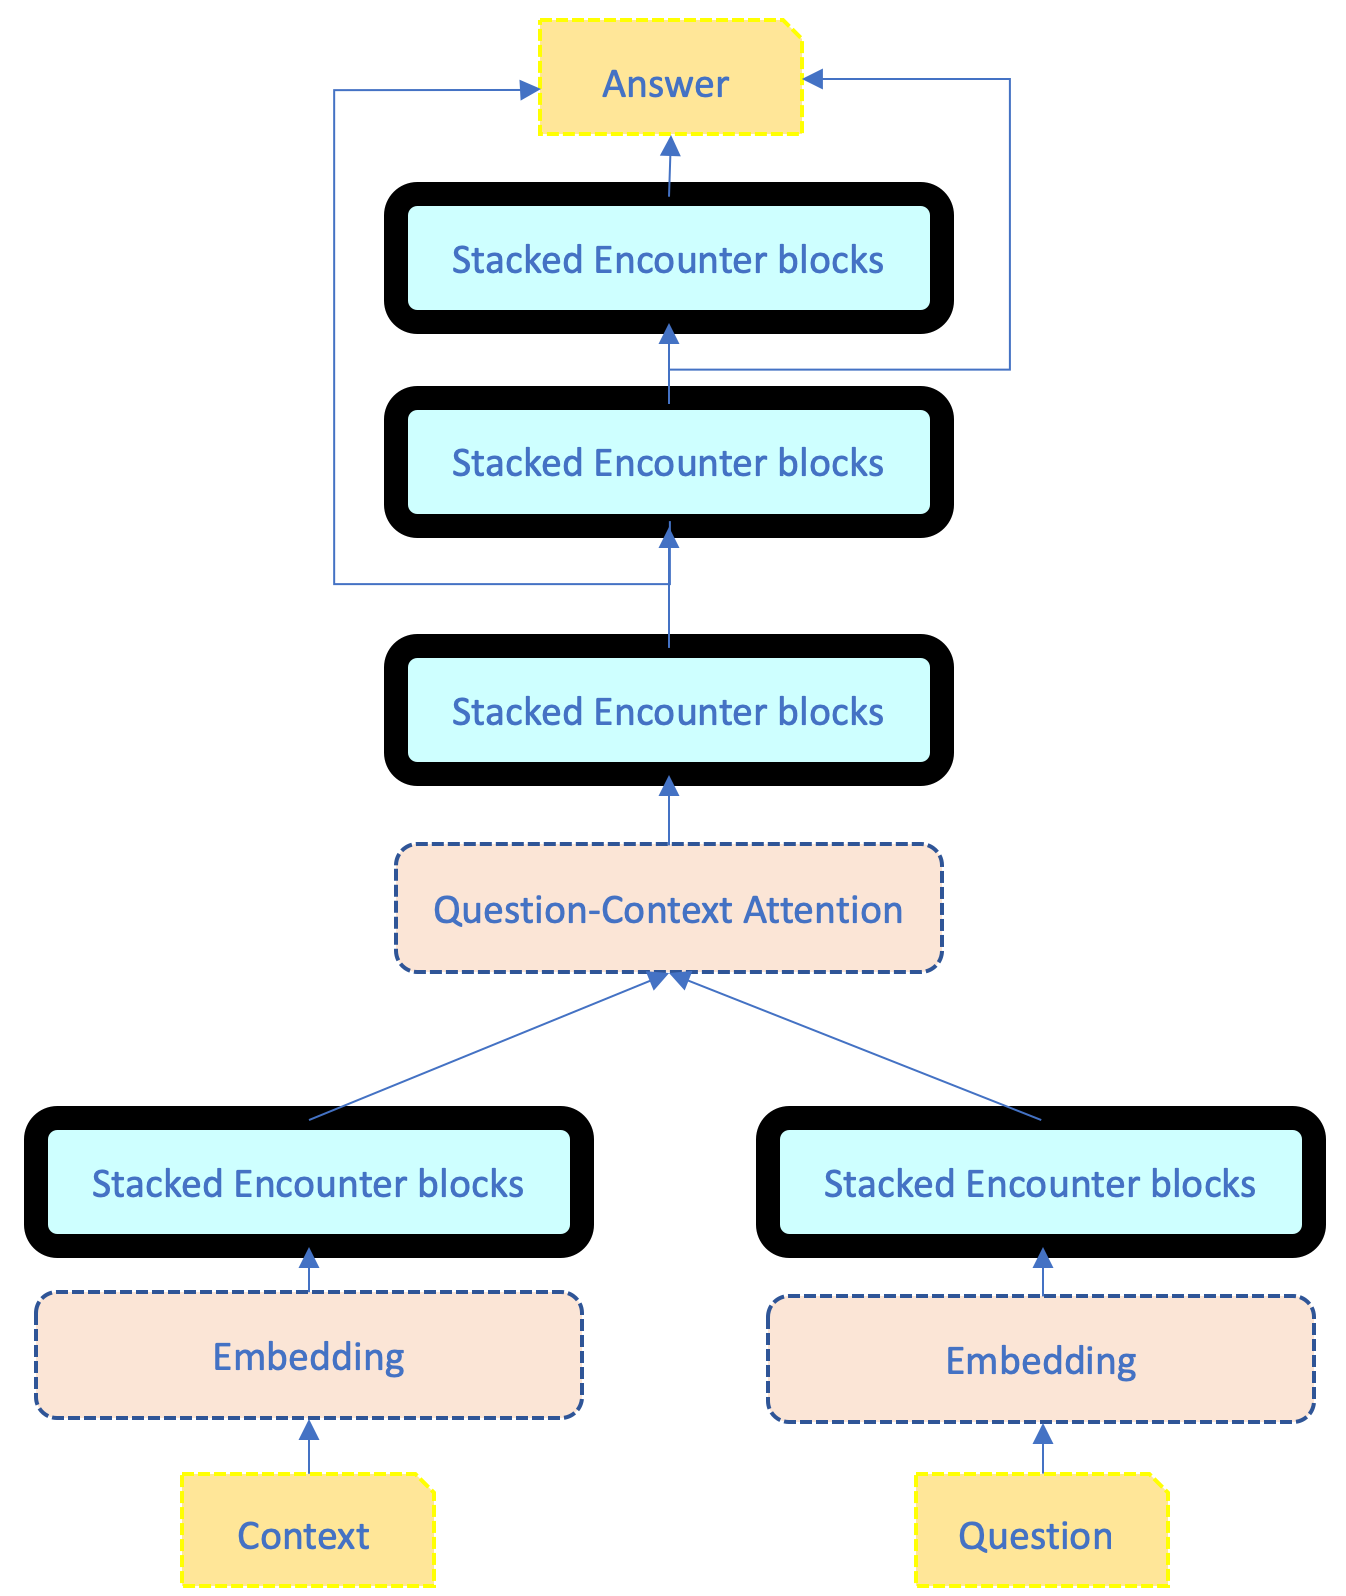
\includegraphics[scale=0.20]{../images/QANet.png}
\caption{\small Overall Model - logical view}
\end{figure}
QANet architecture consists of 5 key modules: an embedding layer, an encoder layer, a context-query attention layer, a modeling layer and an output layer. Embedding layer combines the word and character embeddings into a singular representation for each word. After that, the context and the question are passed through their respective encoder layers. The output from the encoders are fed to the Context-Query attention layer which combines context and query and produces a representation for each word in context. The key layer for prediction is the output layer. Similar to method described in \cite{seo2016bidirectional}, the optimization function is formulated as follows. Let $$P^1 = \textit{softmax}(W_1[M_0 ; M_1]) \qquad P^2 = \textit{softmax}(W_2[M_0 ; M_2])$$ be the probabilities of each position in the context being start and end of the answer span, respectively. 
                                               
Where $W_1$ and $W_2$ are trainable weights and $M_0 , M_1 , M_2$ are outputs from the three model encoders. Now the objective function could be defined as the sum of negative log probabilities of predicted distributions indexed by true start and end indices, averaged over the training instances. $$Log(\theta) = - 1/N \sum_i^N [log(P^1_{{y^1_i}}) + (P^2_{{y^2_i}})]$$
Where $y_i^1$ and $y_i^2$ are start end positions of the $i^{{th}}$  training instance from ground truth. The model outputs probabilities for all pairs similar to other pointer networks for reading comprehension. Through an efficient method (such as using dynamic programming), the best pair of spans $(s,e)$ that maximize $p_s^1 p_e^1$ have to be chosen as the prediction. Ultimately these probabilities are turned into a span consisting of a start index and an end index, indicating the location of the answer in the context paragraphs. Since, the answer is essentially a contiguous phrase in the context, predicting start and end index is sufficient. The overall model is shown below.

\section{Approach}
Our motivation behind choosing this project is to carefully study the key ideas (such as, attention mechanism, pointer networks etc.) from the recent innovations of neural architectures that the QANet is built upon. We hope to gain hands-on experience by implementing the architecture “from the scratch”. So the first step essentially is implementing the architecture. The second step is to perform an error analysis on the development set and come up with a few ideas to implement. At the time of writing this, we are still in the process of training our first implementation and hence we have not explored any ideas fully. At the outset, we want to explore ideas along two different dimensions: 1. Answerability prediction improvements, 2. General accuracy improvements for answerable questions. 

\subsection{Answerability Improvements} To deal with unanswerable cases, systems must learn to identify a wide range of linguistic phenomena such as negation, antonymy and entity changes between the passage and the question. Therefore we expect the performance of the base QANet over SQuAD [2.0] to be worse. Previous works, including the framework supplied as part of the baseline implementation for default final project, usually predict an additional “no-answer” probability to detect unanswerable cases. Given a context of N tokens, this model predicts start/end probabilities for N+1 positions. The start/end probabilities in the extra position are used for answerability prediction. Other approaches include adding auxiliary losses to the system \cite{hu2018read+} or encoding the no-answer option within the model \cite{clark2017simple}.

\subsection{Accuracy Improvements for Answerable Questions} After the error analysis we would explore ways of borrowing some ideas from Transformer-XL architecture \cite{dai2019transformerxl} to improve accuracy of QANet, especially for handling long-range dependencies. 

\section{Experiments}
Currently we are in the process of training our initial implementation. Due to GPU memory constraints we have configured the experiments to run with the following settings: The hidden size of the model is 96 (in contrast to the 128 from the paper). The number of attention heads is set to 1 (instead of 8). Further, batch size is limited to 32 (instead of 64). The running time of the experiments seem to be well in excess of 24 hours and the model learns slowly and we reach EM of 53.2 and F1 score of 55.2. We observe that well into the experiment (after 8 epochs) the NLL (native log-likelihood) loss suddenly starts climbing sharply, indicating some serious issues with our implementation which we are investigating. 

\begin{figure}[h!]
  \centering
  \begin{subfigure}[b]{0.3\linewidth}
    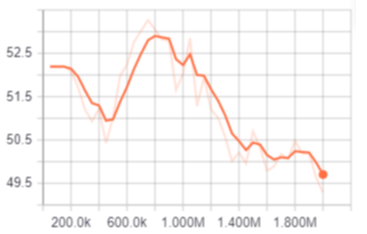
\includegraphics[width=\linewidth]{../images/EM.PNG}
     \caption{EM}
  \end{subfigure}
  \begin{subfigure}[b]{0.3\linewidth}
    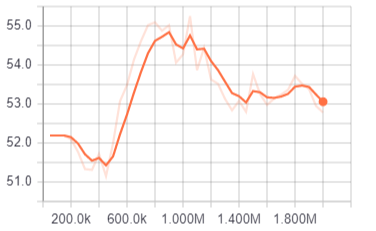
\includegraphics[width=\linewidth]{../images/F1.PNG}
    \caption{F1}
  \end{subfigure}
  \begin{subfigure}[b]{0.3\linewidth}
    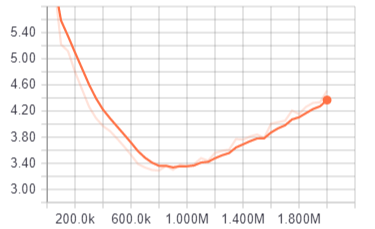
\includegraphics[width=\linewidth]{../images/NLL.PNG}
    \caption{NLL}
  \end{subfigure}  
  \caption{Training run} 
\end{figure} 

\subsection{Data and Evaluation}
We use the usual evaluation metrics for SQuAD - EM (Exact Match) and F1 measure. The baseline for our implementation will the Bi-DAF model supplied as part of the default final project. As a departure from the QANet paper, we have chosen not to re-implement the data-augmentation due to time-constraints; instead, if time permits, we will be evaluating against domain-specific datasets such as CliCR \cite{vsuster2018clicr} to further explore the different comprehension skills (co-reference, tracking, logical etc.) of the system as described in \cite{sugawara2017evaluation}.

\subsection{Results}
Currently we are in the process of training our initial implementation, so no results are available yet. This section will be updated later.

\subsection{Future Work}
The first order of business must be be to make sure that the QANet model learns best to the current specification of the loss function, which is not the case currently.  Once we are able to train the model successfully we will update this section.  

\bibliographystyle{plain}
\bibliography{../References}

\end{document}